\documentclass[12pt]{article}
\usepackage[T1]{fontenc}
%\usepackage[mono=false]{libertine}
%\usepackage{verbatim}
\usepackage{amsmath,amsthm}
\usepackage{amssymb}
\let\circledS\relax % amssymb clashed with mathdesign
\usepackage[charter,cal=cmcal,mono=false]{mathdesign}
\usepackage{inconsolata} % for mono font
\usepackage[b5paper]{geometry}
%\usepackage[paperwidth=5.5in,paperheight=6in,left=0.2in,right=0.2in,top=0.5in,bottom=0.5in]{geometry}
%\usepackage[margin=2.9cm]{geometry}

\usepackage[yyyymmdd]{datetime}
\renewcommand{\dateseparator}{--}

\usepackage{color,braket}

\usepackage{natbib, enumerate}
\usepackage[usenames,dvipsnames,svgnames,table]{xcolor}
\usepackage[colorlinks=true,
            linkcolor=blue,
            urlcolor=black,
            citecolor=gray,backref=page]{hyperref}



\usepackage{graphicx} % add pdf as image
\usepackage{multicol} % two-columns
\usepackage{CJKutf8}



%\usepackage[hyperpageref]{backref}
\DeclareMathOperator*{\argmax}{arg\,max}
\newcommand*{\dif}{\,\mathrm{d}}
\renewcommand*{\u}{\underline}
\newcommand*{\cB}{\mathcal{B}}
\newcommand*{\cN}{\mathcal{N}}
\newcommand*{\inv}{^{-1}}
\newcommand*{\isom}{\cong}


\newtheorem{prp}{Proposition}

\theoremstyle{definition}
\newtheorem{qst}{Question}
\theoremstyle{remark}
\newtheorem*{asw}{Answer}


\begin{document}

\title{A crash course on topology}
\author{Haoran LEI}  
\date{\today}

\maketitle

\begin{CJK}{UTF8}{gkai}
   

\begin{abstract}

  这份讲义草稿起源于我 2021 年春季在湖南大学``挂羊头卖狗肉''讲授的拓扑学课程, 主要受众是理论经济学方向的研究生.
  行文夹叙夹问, 有时像习题集多过像讲义.  

  这份讲义非常不完善, 并且在可预见的未来我都没有时间去修改它. 

  Very preliminary and I am afraid I will not work on it in the near future.
   
\end{abstract}

\end{CJK}

\clearpage
\begin{center}
  \section{Introduction to topological space}
\end{center}

\setcounter{section}{1}
\subsection{Topological spaces}

Topologies are about open sets.
We review some basic properties of a topological space and its connections to a metric space.

\begin{qst}
  Let $(E,d)$ be a metric space. Denote by $\tau$ the collection of subsets of $E$:
  $$
  \tau := \set{A \subseteq E | \forall x\in A, \, \exists r >0 \text{ such that } B(x,r) \subseteq A}. 
  $$
Show that $\tau$ is a topology on set $E$. 
Moreover, we call $\tau$ the {\em topology induced by metric $d$.}  
\end{qst}

\begin{qst}
  Let $(E, \tau)$ be a topological space. 
  Given a subset $F$ of $E$, define $\tau_F := \set{U \cap F | U \in \tau}$. Verify that $\tau_F$ is indeed a topology on $F$.
  Moreover, we call $(F, \tau_F)$ a {\em topological subspace} of $(E, \tau)$. 
\end{qst}

\begin{qst}
  Let $(E,d)$ be a metric space. For a subset $F \subseteq E$, let $d|_F$  be the restriction of metric $d$ on set $F$.
  Denote by $\tau$ and $\tau_F$ the topologies induced by $d$ and $d|_F$ respectively.
  Show that $(F, \tau_F)$ is a topological subspace of $(E, \tau)$.
\end{qst}

\begin{qst}
  Let $E$ be a topological space and let $F$ be a topological subspace of $E$. Suppose that $A \subseteq F$ is closed (or respectively, open) in $F$.
  Illustrate that $A$ may not be closed (or respectively, open) in $E$. [Recall that by definition, if $A \subseteq F$ is open in $E$ then it must be open in $F$.]
\end{qst}


\subsection{Neighborhoods and neighborhood bases}

A neighborhood of $x \in E$ is any set in the topological space that is bigger than some open set $U$ containing $x$.
The collection of all neighborhoods of $x$ is denoted by $\mathcal N(x)$, also formally known as the neighborhood system for $x$.

A neighborhood need not be open.
Those neighborhoods that also happen to be open (or respectively closed) are known as open (or respectively closed) neighborhoods.

The collection of all neighborhoods having a certain "nice" property forms a neighborhood basis,
while these neighborhoods are not necessarily open.
Equivalently, we can define a topology via one of the neighborhood bases.

\begin{qst}
  Given a topological space $E$ and a point $x \in E$, a family of neighborhoods $\mathcal B(x) \subseteq \mathcal N(x)$ is called a {\em neighborhood basis} for $x$ if for each $U \in \mathcal N$, there exists $V \in \mathcal B(x)$ such that $V$ is a subset of $U$.
  \begin{enumerate}[(a)]
    \item Show that the set of all open neighborhoods of $x$ constitute a  neighborhood basis for $x$.
    \item Illustrate that the set of all closed neighborhoods of $x$ may not be a neighborhood basis for $x$.    
  \end{enumerate}
\end{qst}

\begin{qst}
  Show that $U$ is open if and only if $\forall\, x \in U$, $U \in \mathcal N(x)$; that is, $U$ is a neighborhood for all its members. [Hint: consider a neighborhood basis of $x$.]
\end{qst}

The topology on $E$ is determined uniquely by all the neighborhood bases on $E$. Alternatively, we can give an axiomatic description of a topology by specifying the neighborhood bases rather than the open sets.    
\medskip

\noindent {\bf Theorem.} Denote by $E$ be an non-empty set.
For any $x \in E$, denote by $\mathcal B(x)$ a collection of subsets of $E$ that contain $x$. Moreover,
\begin{enumerate}[(B1)]
  \item For any $V \in \mathcal B(x)$, $x \in V$.
  \item For any $(U,V) \in \cB \times \cB$, there exists $W \in \cB (x)$ such that $W \subseteq U \cap V$.
  \item For any $V \in \cB (x)$, these exists $U \subseteq V$ such that (i) $x \in U$ and (ii)  $\forall \, y \in U$, $\exists\, W \in \cB(y)$ such that $W \subseteq U$. 
\end{enumerate}  
Then there exists a unique topology $\tau$ such that for each $x \in E$, $\cB(x)$ is a neighborhood basis for $x$.

\begin{qst}
  Prove the theorem above.\footnote{This problem is hard, but hugely beneficial. You will have a great understanding of neighborhood bases by working on it.
  So before reading the solution, try solving it by yourself. It's also of help to stay puzzled for days with a great theorem like this.}
\end{qst}


\subsection{Hausdorff space}
A topological space $E$ is called a {\em Hausdorff space} (or separable space) if for all $(x,y) \in E \times E$ with $x \neq y$, there exist a neighborhood of $x$, denoted by $U$, and a neighborhood of $y$, denoted by $V$, such that $U \cap V = \emptyset$.
Hausdorff spaces are widely used in analysis because a sequence $(x_n)$ in a Hausdorff space cannot have more than one limit. 
You will learn what is a limit in a topological space and how to prove that claim in the next class.    

\begin{qst}
  For $x \in E$, denote by  $\mathcal{CN}(x)$ the collection of closed neighborhoods of $x$.
  \begin{enumerate}[(a)]
    \item  
    Given a topological space $E$, show that $E$ is a Hausdorff space iff 
    $$
    \bigcap_{A \,\in\, \mathcal{CN}(x)} A = \set{x};
    $$
    that is, the intersection of all the closed neighborhoods of $x$ yields the singleton $\set{x}$. 
    \item A corollary of (a) is that if $E$ is a Hausdorff space, then
    $$
    \bigcap_{A \,\in\, \mathcal{N}(x)} A = \set{x}.
    $$ 
    Illustrate that the converse may not hold. [Hint: Some imagination beyond the usual topology on $\mathbb R$ may be needed.]
  \end{enumerate}

\end{qst}


\clearpage
\begin{center}
  \section{Limits, nets and homeomorphisms}
\end{center}

\setcounter{section}{2}
\begin{qst}[A classical counterexample of non-Hausdorff space]
Let $R^* = \mathbb R \setminus \set{0}$ and $E = R^* \cup \set{-\infty,+\infty}$. A set $A \subseteq E$ is open if it satisfies
\begin{enumerate}[i.]
  \item $A \cap R^*$ is open in the topological space $R^*$ endowed with the usual topology, and 
  \item if $+\infty \in A$ or $-\infty \in A$, then $A$ includes some set   $R^* \cap U$ where $U$ is a neighborhood of $0$ in $\mathbb R$.
\end{enumerate}
Show that:
\begin{enumerate}[(a)]
  \item The collection of sets that satisfy conditions (i) and (ii) constitute a topology. Denote the topological space by $(E,\tau)$.
  \item The topological space $(E,\tau)$ is non-Hausdorff.
  \item The intersection of all neighborhoods of $x \in E$ is $\set{x}$. That is,
     $\bigcap_{V \in \cN(x)} V = \{x\}$ for all $x \in E$. [Hint: What are the closed sets in $E$?] 
\end{enumerate}  
\end{qst}


\subsection{The closure and the interior}

Denote by $E$ a topological space and let $A \subset E$. 
A point $x \in E$ is called an
\textit{adherent point}\footnote{Also known as closure point or contact point.}
of set $A$ if every neighborhood of $x$  
contains at least one point of $A$.
In addition, if every neighborhood of $x$  
contains at least one point of $A$ different from $x$, 
it is called a \textit{limit point} of set $A$. 

\begin{qst}
  Denote by $\bar A$ the set of all adherent points of $A$.
\begin{enumerate}[(a)]
  \item Show that $\bar A$ is closed.
  \item Show that $A \subseteq \bar A$.
  \item Show that $\bar A$ is the smallest closed set that contains $A$. [For that reason, $\bar A$ is also called the closure of $A$.]
\end{enumerate} 
\end{qst}

\begin{asw}
  
\end{asw}


A point $x \in E$ is called an interior point of $A$ if there exists a neighborhood $U$ of $x$ such that $U \subseteq A$.
Denote by $\mathring A$ the set of its interior points.
Formally $\mathring A$ is known as the interior of set $A$.

\begin{qst}
  \begin{enumerate}[(a)]
    \item Show that $\mathring A \subset A$.
    \item Show that $\mathring A$ is open. 
    \item Show that $\mathring A$ is the largest open set included in $A$.
    \item Show that $A$ is open if and only if $\mathring A = A$.   
  \end{enumerate} 
\end{qst} 

\begin{asw}
  
\end{asw}

The following are useful properties of the closure and interior of set $A$. Proving them is also an incredible chance to review the language of basic topology (e.g.\ open and closed sets, neighborhoods, and the set operations on them....) 

\begin{qst}
  \begin{enumerate}[(a)]
    \item Show that $\mathring{A}=\mathring{\mathring{A}}$ and $\bar A = \bar{\bar{A}}$.
    \item Show that $E \setminus \mathring A = \overline{E \setminus A}.$
    \item Show that $\bar A \cup \bar B = \overline{A \cup B}$ and 
      $\mathring A \cap \mathring B = \mathring{\widehat{A \cap B}}$ where 
      $\mathring{\widehat{A \cap B}}$ is the interior of the intersection of $A$ and $B$. 
  \end{enumerate} 
\end{qst} 

\subsection{Limits of a  sequence v.s.\ limit points of a set}

Given a sequence $(x_n)_{n \in \mathbb N}$ in $(E, \tau)$,
we say $x \in E$ is a \textit{limit} of $(x_n)$ if for any neighborhood $V$ of $x$, there exists some $N$ such that $x_n \in V$ for all $n>N$.
A sequence $(x_n)$ need not have a limit; and when it has, it can have multiple limits.
We say $(x_n)$ in $(E, \tau)$ is \textit{convergent} if it approaches some limit $x \in E$, formally written as $\tau \text{-} \lim_{n\to\infty} x_n = x$. We use the shorthand $\lim_{n\to\infty} x_n$ (i.e.\ dropping the $\tau$ beforehand)  when there's no ambiguity.

\begin{qst}
  Let $E = \set{a,b,c}$ endowed with a topology 
  $$\tau = \big\{ \set{a,b},\set{b,c}, \set{b}, E, \emptyset \big\},$$
  \begin{enumerate}[(a)]
    \item What are the limit points (if any) of $(x_n)$ where $x_n = b$ for each $n$? 
    \item Is $(E,\tau)$ a Hausdorff space?
    \item Show that if $(E,\tau)$ is a topological space, then any convergent sequence in $E$ has a unique limit.
  \end{enumerate}
\end{qst}

\medskip

You may wonder whether we can use the \textit{limits of each sequence} $(x_n)$ in $A \subseteq E$ to get the \textit{limit points of} $E$.
However, this does not hold in a general topological space.

\begin{qst}[cocountable topology] 
Let $E = R$ and call a set $A \subseteq E$ open if $A^c$ is countable.
\begin{enumerate}[(a)]
  \item Show that the set of ``open sets'' defined above constitute a topology. 
   
  Denote the topology by $\tau$.
  
  \item Show that in $(E, \tau)$ a sequence $(x_n)$ is convergent if and only if $x_n$ is a constant after some $x_N$. 
  \item Illustrate that there exists some set $A \subset E$ whose limit points cannot be approached by any sequence in $A$.
\end{enumerate}  
\end{qst}

\subsection{Nets}


Plain sequences detect topological properties in metric spaces, but they fail to do so in more general topological spaces.
That motivates the concept of \textit{nets}.\footnote{A great introduction to nets can be found at nLab: \url{https://ncatlab.org/nlab/show/net}.}
A net is a function $\nu$ from a special preordered set $D$ to the topological set $E$.


\noindent \textbf{Definition [Directed set].}
A \textit{directed set} is a preordered set $(D, \le)$
\footnote{Here $D$ is equipped with a reflexive and transitive relation. For a  concrete example, think of $\le$ as the preference relation.}
such that every finite subset has an upper bound. That is,  for any
$a,b \in D$ there exists $c \in D$ 
such that $a \le c$ and $b \le c$.

Examples of directed sets include 
a directed set of natural numbers and a directed set of neighborhoods.
Specifically, let $A_{\ge}$ and  $B_{\ge}$ be directed sets.
Then the Cartesian product $A \times B$ of the underlying sets becomes itself a directed set by setting
$$
(a_1, b_1) \leq (a_2, b_2) \text{ if } a_1 \le a_2, b_1 \le b_2
$$


\noindent \textbf{Definition [Nets].}
A net in a set $X$ is
\begin{enumerate}
  \item  a directed set $A$, called the index set, and
  \item  a function $\nu \colon A \to X$, from the underlying set $A$ to $X$.
\end{enumerate}
We say $\nu$ is a net and set $A$ indexes the net.
For example, a sequence is a net whose directed set of indices is the natural numbers. 
Since $A$ is a preordered set, it makes sense to talk like ``For any neighborhood $U$ of $x$, there exists $i \in A$ such that for all $j \ge i$ we have $v_j \in U$.''
A directed set $A$ is a natural extension of $\mathbb N$, 
and we use $A$ rather than $\mathbb N$ to index a set.


Consider net $\nu: A \to X$ and given a subset $S \subset X$. We say that\footnote{Sometimes one says `infinitely often' in place of `frequently' and even `cofinitely often' in place of `eventually.'
These derive from the special case of sequences, where they may be taken literally.}
\begin{enumerate}
  \item $\nu$ is \textit{eventually} in $S$ if there exists $i \in A$ such that $\nu_j \in S$ for each $j \ge i$.
  \item $\nu$ is \textit{frequently} in $S$ if for every index    $i \in A$ there exists some $j \ge i$ such that $\nu_j \in S$.
\end{enumerate}

I will not go into the details here. Instead, I urge you to read the exposition of nets at nLab.
A beautiful result is that a topological space $(E,\tau)$ is compact if and only if every net in $X$ has a sub-net that converges.


\subsection{Continuous mappings and homeomorphisms}

Given two topological spaces $E$ and $F$ and a mapping $f: E \to Y$, let $x \in E$ and denote its image by $f(x)$.
We say $f$ is continuous at $x \in E$ if for any neighborhood $V$ of $f(x)$, 
the inverse image of $V$, $f^{-1}(V)$ is a neighborhood of $x$.
We say $f$ is continuous on $E$ if it is continuous at each $x \in E$.

If you do not like the usage of neighborhoods and prefer using open sets, 
an equivalent definition is that $f \colon E \to F$ is open on $E$ 
if $f \inv (O)$ is open for each open set $O \subseteq F$.
You are asked to prove that in Question \ref{qst:conti}.

\begin{qst} \label{qst:conti}
  Let $E$ and $F$ be two topological spaces and $f: E\to F$ be a mapping from $E$ to $F$. Show that the following statements are equivalent:
  \begin{enumerate}
    \item $f$ is continuous on $E$
    \item $f \inv (O)$ is open for each open set $O \subseteq F$
    \item $f \inv (A)$ is closed for each closed set $A \subseteq F$ 
  \end{enumerate}
\end{qst} 

Continuous mappings are nice animals. The composition of two continuous mappings is still continuous.
As the continuity of $f$ depends on the topologies on $E$ and $F$,
you can trick your calculus teacher by claiming that every real function is continuous! As long as you equip $R$ with the strongest topology --- discrete topology.


Given two topological spaces $E$ and $F$, we say they are \textit{homeomorphic}
if there exists some bijection $f: E \to F$ such that both $f$ and
$f \inv$ are continuous. We call such $f$ a \textit{homeomorphism}  between the two topological spaces $E$ and $F$.

Homeomorphism is the `isomorphism' between topological spaces.
Two homeomorphic topological spaces are basically the same for the purposes of topology.
A left and right glove are identical, because the left-right reflection is continuous in both directions. The difference between the left and right gloves isn't intrinsic to the gloves themselves, but is in the way the gloves are embedded in three-dimensional space.
Another classic example is the
cup--donut topological equivalence. 
Imagine continuous mappings as deformations of elastic physical bodies, which may be deformed by stretching them without tearing.
By doing that, you can turn a coffee cup to a donut (or formally, a torus). 

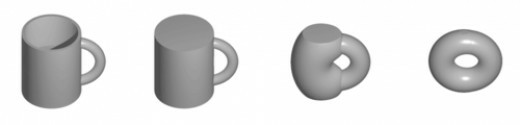
\includegraphics[width=\textwidth]{cup.jpg}

\begin{qst} Consider $\mathbb R$ endowed with the usual topology.
  \begin{enumerate}[(a)]
    \item Prove that any open interval $(a,b)$ is homeomorphic to the interval $(0,1)$. Here both $a$ and $b$ can be infinite. 
    \item Prove that any two bounded closed intervals of the real line are homeomorphic; i.e., $[a,b]$ is homeomorphic to $[0,1]$.  
    \item Show that if we drop out `bounded,' the statement above does not hold. [Hint: compactness]
  \end{enumerate}
\end{qst}



\subsubsection{From homeomorphism to knot theory}

I cannot help but talk more about these embedding stuff.
Consider this analogy: The symbol \texttt{b} can be turned into \texttt{d}, 
but to do it you have to lift the b out of the plane and flip it over. If you leave b and d embedded in the plane you can never turn one into the other (although you can turn b into q and d into p). 
So the difference is not in the shapes \textit{themselves}
but in the way they inhabit the plane.
Left and right gloves are distinguishable if they remain in three-dimensional space.
But in larger spaces, they're identical. It's easy to turn a left glove into a right glove if you can lift it into four-dimensional space and flip it over.

The branch of topology called ``knot theory'' concerns the way simple shapes like circles can be embedded into three dimensions.
Topologically a knotted loop of string and an unknotted one are the same --- but again, their embeddings into three-dimensional space are different. 


\includegraphics[width=0.8\textwidth]{knots}


Dealing with this topologically requires extra efforts.
One embeds the knotted loop in space and then considers whether there is a continuous deformation of the entire space, including the loop, that transforms the knotted loop into the unknotted one. Viewed in this way one can say that a trefoil knot (shown in the image) is chiral, 
because although each is topologically equivalent to a plain circle, the left-handed trefoil knot can never be smoothly transformed into the right-handed one
without removing it from three-dimensional space.

So next time do not leave a bad review when you receive a pair of left-hand gloves. They are actually the same with right-hand gloves! 
After all, according to some really smart physicists the universe we inhabit is made of 11 dimensions.


\begin{qst}
  Consider the coffee mug and torus example. Is the coffee mug shown in the image
  chiral? How about the torus?
\end{qst}

\begin{asw}
  A coffee mug is \textit{not} chiral in the topological sense. 
  It has a handle on the left side, and we can deform space to move the handle to the right side instead: just turn the cup around, now the handle is on the other side. No fourth dimension is required. 
  There are also many other ways to get the handle to the other side.
\end{asw}

\begin{qst}[Just for fun]
  Is a ball (sphere + interior) being equivalent to a (solid) cube? 
  A topologist answers yes and an algebraist answers no. Explain the differences.
\end{qst}

\begin{asw}
  Topology is ``geometry minus shape.'' That is, we topologists are completely ignoring the exact shape of an object.   Topological equivalence only cares about preserving a special closeness relation (i.e.\ homeomorphism) between the points of an object.
  So a ball is equivalent to a cube.

  They algebraists care about the group of symmetries.
  The sphere having infinitely many symmetries, while a cube only has a finite symmetry group.
\end{asw}





\clearpage
\begin{center}
  \section{Compact spaces, Hausdorff spaces, and Locally compact Hausdorff spaces}
\end{center}

\subsection{Compact spaces}

Compactness is an amazing analytical notion expressed in 
topologian.
A topological space 
is compact if all sequences (or more generally, nets) inside it converge as much as possible.
Compactness is a topological notion that was developed to abstract the key property of a subspace of a Euclidean space being closed and bounded: every net must accumulate somewhere in the subspace.
Roughly, the reason is that boundedness implies that
the net cannot escape the subspace, and the point to which it accumulates lies in the subspace by closure. 
This is the statement of the Heine-Borel theorem as you may have seen in calculus.



Compactness provides an \textit{intrinsic} way of formulating this bounded-and-closed property in the context of general topological spaces, without the need to view them as subspaces of an ambient space.
Still, it is common to work with compact subsets of a given space. These are those subsets which are compact spaces with the subspace topology 
(see Question \ref{qst:subspace}).


There are many ways to say that a space $E$ is compact.
The first is perhaps the most common.

\subsubsection{Open covers}

Denote by $E$ a topological space. We say $E$ is \textit{compact} if for any open cover $\set{O_i}_{i \in I}$ with
$\cup_{i \in I} O_i = E$, there exists a finite subcover
$\set{O_j}_{j \in J}$ such that 
$\cup_{j \in J} O_j = E$.
Put in plain English,
a topological space is compact if every open cover has a finite subcover.




An equivalent definition is that for any family of closed sets $\set{F_i}_{i \in I}$ with $\cap_{i \in I} F_i = \emptyset$, there exists $\{F_j\}_{j \in J}$ such that
$\cap_{j \in J} F_j = \emptyset$.
Taking the contrapositive,
if  
\begin{equation}
\cap_{j \in J} F_j \neq \emptyset \text{ for any finite }
\{F_j\}_{j \in J},  
\end{equation}
then the intersection of the set family  
cannot be empty:
$\cap_{i \in I} F_i \neq \emptyset$.

Display (1) is called the \textit{finite intersection property.}
One corollary  of the equivalent definition --- the nested intervals theorem --- is used often in calculus.

\begin{qst}
   Let $E$ be a topological space. Show that if $(F_n)_{n \ge 1}$ is a sequence of nonempty closed sets with $F_n \subseteq F_{n-1}$,
   then $$ \cap_{n \ge 1} F_n \neq \emptyset. $$
\end{qst}  


Usually we wish to determine whether $F \subseteq E$ is 
compact or not, and
we can still use the open covers in $E$ to detect whether 
$F$ is compact or not.

\medskip
\noindent \textbf{Theorem.} Denote by $E$ a topological space and $F\subseteq E$ a subspace.
Then $F$ is compact if and only if
for any open covers of $F$ in $E$, there is a finite subcover.



\begin{qst}\label{qst:subspace}
  Formulate the plain English in the theorem above and
  prove it.
\end{qst}

\subsubsection{Other definitions}


In another direction, the definition of a compact topological space also works for locales.
We can also define
compactness via ultrafilter convergence.
Moreover, A uniform space 
$E$ s compact if and only if it is complete and totally bounded. 
Finally, 
category theorists live in their own world and formulate
compactness using stability properties.
We refer interested readers to nLab:
\url{https://ncatlab.org/nlab/show/compact+space}.

\subsection{Compactum}


Hausdorff spaces (aka ``compacta'') are nice animals.
In a compact Hausdorff space (aka ``compactum''),
every limit of a sequence or more generally of a net that should exist does exist (as it is compact) and does so uniquely (as it is Hausdorff).
Mathematicians love Hausdorff spaces so much that a special name ---compacta/a compactum --- is given to them.\footnote{Indeed, some authors even use ``compact'' to mean ``compact and Hausdorff,''
and use the word ``quasicompact'' to refer to just ``compact'' as we are using it here. 
This custom seems to be prevalent among algebraic geometers, and particularly so within French mathematicians or guys who speak French.}

\begin{qst}\label{qst:compact-closed}
  Denote by $E$ a Hausdorff space and $F \subseteq E$ a  subspce of $E$.
  \begin{enumerate}[(a)]
    \item Show that $F$ is a Hausdorff space.
    \item Show that $F$ is compact $\implies$ $F$ is closed. [Hint one: You need to show $F^c$ is open. Hint two: Show that for each $x$ in $F^c$ there is an open ball in it containing $x$. Note that $F$ is a compactum now!]
    \item Assume furthermore that $E$ is compact. Show that    $F$ is compact $\iff$ $F$ is closed. [Hint: Use the finite intersection property.]
  \end{enumerate}
\end{qst}

%
%\begin{asw}
%  (a) Let $x,y \in F$ and $x \neq y$. 
%      Since $E$ is Hausdorff, there exist two disjoint open sets $U, V \subseteq E$ such that $x \in U$ and $y \in V$.
%      Hence $U \cap F$ and $V \cap F$ are open in $F$ and contain $x$ and $y$ respectively.
%
%  (b)   
%\end{asw}

In $\mathbb R^n$, a set is compact iff it is closed and bounded.
We are interested in the relationship between being compact and closed
(since boundedness is not defined in a topological space).
Question \ref{qst:compact-closed} implies that if a topological space $F$ inhabits a larger Hausdorff space $E$,
then compactness implies closedness.
Moreover, if it inhabits a compactum (i.e.\ being both compact and Hausdorff),
then compactness is the same as closedness.

In general, neither compactness nor closedness implies the other.
See the question below for examples.

\begin{qst}
   Verify the following examples.
   \begin{enumerate}[(a)]
     \item In a topological space with finitely many open sets, each set is compact. For example, the indiscrete/trivial topology.
     \item Endow $R$ with the co-finite topology, in which
        a set is open if and only if its complement is finite. Clearly $N$ is neither open nor closed. 
        Show that $N$ is compact. Indeed, \textit{every} subset is compact in this topology.
     \item Consider \textit{the line with two origins:}
        $E = [-1,0) \cup \set{a,b} \cup (0,1]$. The set 
        $[-1,0) \cup \set{a} \cup (0,1]$ is compact but not closed. Its closure includes point $b$.
   \end{enumerate}
\end{qst}

\subsection{Locally compact Hausdorff space}

Analysts usually work in Hausdorff space, but not so often in compact space (e.g., $\mathbb R$ is non-compact).
Assuming we only talk about stuff in Hausdorff space,
local compactness is
a useful but weaker notion than compactness.
For example, given a compact Hausdorff space $E$,
its subspace $F$ may not be compact but it must be locally compact.


A Hausdorff space $E$ is \textit{locally compact} if every point has a compact neighborhood.
If $E$ is non-Hausdorff, then being locally compact requires each point to have a compact neighborhood basis ---
a neighborhood basis consisting of compact neighborhoods --- which is a stronger condition.
The second definition of local compactness is not used much as we pay little attention to non-Hausdorff space.

\begin{qst}
  Let $E$ be a Hausdorff space. If $E$ is locally compact, then for each $x \in E$ there exists a neighborhood basis consisting of compact neighborhoods for $x$.
\end{qst}

%\begin{asw}
%  Let 
%\end{asw}


In mathematical analysis locally compact spaces that are Hausdorff are of particular interest, which are abbreviated as LCH spaces.
Examples of locally compact Hausdorff spaces that are not compact include:
\begin{itemize}
  \item The Euclidean spaces $\mathbb R^n$, which are are locally compact as a consequence of the Heine--Borel theorem.
  \item All discrete spaces are locally compact and Hausdorff. These are compact only if they are finite.
  \item All open or closed subsets of a locally compact Hausdorff space are locally compact in the subspace topology. This provides several examples of locally compact subsets of Euclidean spaces, such as the open unit ball.

 
\end{itemize}



\clearpage
\begin{center}
  \section{Product topology}
\end{center}

\setcounter{section}{4}

This lecture is about product topology.
There are three important ways of creating new topological spaces from old ones:
forming subspaces, quotient spaces, and product spaces. We focus on product topology today.

\subsection{The product topology: Finite products}


Let $(X, \tau)$ be a topological space.
A collection $\mathcal B$ of open sets of $X$ is said to be a \textit{basis for the topology} $\tau$ if
every open set is a union of members of $\mathcal B$.
So $\mathcal B$ generates the topology $\tau$
in the following sense: if we are told what sets are members of $\mathcal B$, then we can determine the members of
$\tau$ --- they are just all the sets which are unions of members of $\mathcal B$.

Not any collection $\mathcal B$ can form a basis for a topology.

\begin{qst}\label{qst:basis}
  Let $X$ be a non-empty set and let $\mathcal B$ be a collection of subsets of $X$.
  Then $\mathcal B$ is a basis for a topology on $X$ iff (i) $\cup_{B \in \mathcal B} B = X$ and (ii) for all $B_1,B_2 \in \mathcal B$,  $B_1 \cap B_2$ is a member of $\mathcal B$. 
\end{qst}

We use the notion of topology basis to characterize the product topology.


\noindent \textbf{Definition.} 
Let $(X_1, \tau_1)$, $(X_2, \tau_2)$,..., $(X_n, \tau_n)$ be topological spaces.
Then the product topology $\tau$ on the set
$X_1 \times \dots \times X_n$ is the topology having the family $\set{O_1\times \dots \times O_n \colon O_i \in \tau_i}$ as a basis.

\begin{qst}
  Show that the family defined in the above definition constitutes a basis. [Hint: use the result of Question \ref{qst:basis}.]
\end{qst}

An obvious (but incorrect!) candidate for $\tau$
is the set of all sets $O_1 \times ... \times O_n$
where $O_i \in \tau_i$. Unfortunately this is not a topology.

\begin{qst}
  Illustrate that the set of all sets $O_1 \times ... \times O_n$ where $O_i \in \tau_i$ may not be a topology.
\end{qst}
\begin{asw}
  Consider $n=2$ and $X_1 = X_2 = \mathbb R$. The topology defined above does not include the union of
  $(0,1) \times (0,1)$ and $(2,3) \times (2,3)$,
  since this is not $O_1 \times O_2$ for any
  choice of $O_1$ and $O_2$.
\end{asw}

\subsubsection{Projections onto factors of a product}


Recall that given two topologies $\tau_1$ and $\tau_2$ on a set $E$,
$\tau_1$ is said to be \textit{finer} than
$\tau_2$ if $\tau_1 \supseteq  \tau_2$.
For example,
the usual topology on $\mathbb R$ is finer than the
cofinite topology on $\mathbb R$.

Let $(X, \tau_1)$ and $(Y, \tau_2)$ be two topological spaces
and $f$ a mapping from $X$ to $Y$.
Then $f$ is called an open (or rep.\ closed) mapping if for every open (or rep.\ closed) set 
$U$ in $X$, $f(U)$ is open (or rep.\ closed) in $Y$.

\begin{qst}
  Show that $f \colon X \to Y$ being $x \in $ \{open, closed, continuous\} does not imply that it is $y \in$ \{open/closed/closed\} $\setminus \set{x}$.
\end{qst}


Product topology is a nice construction.
Indeed, it is the coarsest topology such that each projection is continuous.


\begin{qst}
Let $(X_1, \tau_1)$, ..., $(X_n, \tau_n)$ be topological spaces and $(X_1 \times \dots \times X_n, \tau)$ their topological space.
For each $i \in \set{1,\dots,n}$, let
$$
p_i \colon X_1 \times \dots \times X_n \to X_i
$$
be the projection mapping; that is,
$p_i( \langle x_1, ..., x_n \rangle  ) = x_i$. Show that
\begin{enumerate}[(a)]
  \item each $p_i$ is a continuous surjective open mapping, and
  \item  $\tau$ is the coarsest topology on the set $X_1 \times \dots \times X_n$ such that each $p_i$ is continuous.
\end{enumerate}
\end{qst}

Given topological spaces $X_1, ..., X_n$, 
the product topology can be defined as the
coarsest topology on $X$ such that each projection is continuous.
This observation is of greater significance in the
discussion of products of an infinite number of topological spaces.

\subsubsection{Tychonoff's theorem}

Tychonoff’s Theorem states that if each $(X_i,\tau_i)$ is compact, then $(X, \tau)$ is compact.
Proving Tychonoff’s Theorem for a general product topology is hard.



\begin{qst}
  Prove the Tychonoff’s Theorem for the product of finite topological spaces. Does the inverse also hold?
\end{qst}

An application of Tychonoff’s Theorem is the 
Heine-Borel Theorem in $\mathbb R^n$. 
A set in $\mathbb R^n$ is compact iff
its projection at each dimension is bounded and closed; that is, the set itself is
bounded and closed.  


\subsubsection{Remarks}

The easiest case of product topology is that of finite products. 
Next we study countably infinite products and then the general case.
The most important result is Tychonoff's theorem.

For those who know some category theory, we observe that the category of
topological spaces and continuous mappings has both products and coproducts.
The products in the category are indeed the products of the topological spaces.
You may care to identify the coproducts.


%% This is a bonus section about proving the fundamental theorem of algebra using topology. 


\subsection{The product topology: countably infinite case}

Intuitively, a curve shall have zero area.
One will be amazing to know the existence of space-filling curves.
We attack the topic of space-filling curves using a
curious space known as Cantor space. 
As an added bonus, you will also have a better understanding of the unit interval $[0,1]$.

From a broader perspective,
in this section we extend our study to countably infinite products
of topological spaces.
In this bigger picture space-filling curves is nothing but one example.

\subsubsection{The product topology}

Let $(X_1, \tau_1), \dots, (X_n, \tau_n), ...$ be a sequence of topological spaces.
The product topology of $\prod X_i$ has the following family as its basis:
$$
\set{ \prod O_i \colon O_i \in \tau_i \text{ for all $i \in \mathbb N$ and $O_i = X_i$ for all but a finite number of }i}.
$$

So a basic open set is of the form: 
$$O_1 \times \dots \times O_n \times X_{n+1} \times X_{n+2} \times \dots .$$

It should be noted that a product of open sets in $X_i$ need not be open in $\prod X_i$. 
For example,  let $X_i = \mathbb R$ and then $(0,1)^\infty :=\prod (0,1)$ is not open in $\mathbb R ^\infty$.

Why, you may (and you should) ask, do we define the product topology in this way?
The answer is that only in this way can we guarantee that the product of compact sets is still compact (Tychonoff's Theorem).

For example, consider the box topology $\tau'$ on $\prod X_i$ that has 
$$\set{\prod_{i=1}^\infty  O_i \colon O_i \in \tau_i \text{ for all }i \in \mathbb N} $$
as its basis.
If each $X_i$ is a finite set with discrete topology, 
then $(\prod X_i, \tau')$ is an infinite discrete space. Moreover, each $X_i$ is compact in $(X_i, \tau_i)$ but
$\prod X_i$ is not compact in $(\prod X_i, \tau')$. 
 

There is another justification, which says the product topology is the coarsest
topology on $\prod X_i$ such that each projection mapping
$p_i \colon X \to X_i$ is continuous. 
The proof is left as an exercise.




\begin{qst}
Let $(X_1, \tau_1), \dots,..., (X_n, \tau_n), \dots$ be a sequence of topological spaces and $(X, \tau)$ be their product space. For each $i$, let $p_i \colon \prod_{j=1}^\infty X_j \to X_i$ be the projection mapping:
$$
p_i (x_1,...x_n,...) = x_i.
$$
Show that
\begin{enumerate}[(a)]
  \item each $p_i$ is a continuous, onto and open mapping;
  \item the product topology $\tau$ is the coarsest topology such that each $p_i$ is continuous.
\end{enumerate}
\end{qst}



\subsubsection{The Cantor space and the Hilbert cube}
The Cantor set $G \subseteq \mathbb R$ is closed, uncountable and of measure zero. 
Arm it with the subspace topology,
we obtain the Cantor space $(G,\tau)$.
We are to show that it is homeomorphic (Tóng Pēi) to a countably infinite product of two-point spaces.


For each $i$, let $(A_i, \tau_i)$ be the set $\set{0,2}$ with the discrete topology. Let $A := \prod A_i$ and
consider the product topology $(A,\tau')$.
Then the map 
\begin{align*}
  f \colon &(G,\tau) \to (A, \tau') \\
           &\sum_{n=1}^\infty \frac{a_n}{3^n} \mapsto (a_1,...a_n,...)
\end{align*}
is a homeomorphism.
Here $\sum_{n=1}^\infty \frac{a_n}{3^n}$ is the ternary representation of a number from the Cantor set.


\begin{qst}
  Show that $f$ is indeed a homeomorphism. That is, it is bijective and continuous.
\end{qst}

\begin{asw}
The properties of Cantor set $G$ imply that $f$ is bijective. As $(G, \tau)$ is compact and $(A, \tau')$ is Hausdorff, $f$ is a homeomorphism if it is continuous.
It's sufficient to show that for any \textit{basic} open set
$U = U_1 \times \dots \times U_N \times A_{N+1} \times A_{N+2} \times \dots$ and any
$a = (a_1,a_2,...) \in U$, 

Consider the open interval
$(\sum_{n=1}^\infty \frac{a_n}{3^n} - \frac{1}{3^{N+2}},  
\sum_{n=1}^\infty \frac{a_n}{3^n} + \frac{1}{3^{N+2}} )$
and let $W$ be the intersection of this open interval with $G$. We have $f(W) \subset U$. \qed
\end{asw}

We showed that the Cantor space is topologically the same with the product space $\set{0,2}^\infty$.
We also suggested that any product of compact spaces is still compact.
From the question above, 
we can show that the product of a countable number of homeomorphic copies of the Cantor Space is homeomorphic to the Cantor Space, and hence is compact.

\begin{prp}
  Let $(G_i, \tau_i)$ be a sequence of topological spaces
  each of which is homeomorphic to the Cantor space $(G,\tau)$. Then
  $$
  (G,\tau) \isom \prod_{i=1}^\infty (G_i, \tau_i) \prod_{i=1}^n (G_i, \tau_i)
  $$
\end{prp}





\newpage

\subsection{The product topology: uncountably infinite case}


Let $I$ be a index set and consider 
$ \set{(E_i, \tau_i) : i \in I}$.
The product space, denoted by $\prod_{i \in I} (X_i, \tau_i)$ consists of the product set and the topology $\tau$ having as its basis the family
$$
\mathcal B = \set{ \prod_{i \in I} O_i: O_i \in \tau_i \text{ and } O_i = X_i \text{ for all but a finite number of } i}.
$$
The topology $\tau$ is called the product topology (or the Tychonoff topology).


\paragraph{Remark.} Although we have defined the product topology
rather differently to the way we did when $I$ was 
infinite or finite,
you should be able to convince
yourself that when $I$ is finite the new definition is equivalent to
our previous ones.


We claim that the Tychonoff theorem still holds but withdraws the proof here.
Interested readers may check a free online book
\textit{Topology Without Tears} by Sidney Morris.



\end{document}























